\documentclass[tikz,border=5pt]{standalone}
\usepackage{luatexja}
\usepackage[hiragino-pron]{luatexja-preset}
\usepackage{amsmath,amssymb}
\usepackage{pgfplots}
\pgfplotsset{compat=1.18}
\usetikzlibrary{arrows.meta,calc,decorations.markings,patterns,positioning}

% Common styles
\tikzset{
  axis/.style={-{Stealth[length=6pt]}, thick},
  curve/.style={thick, red},
  dashed curve/.style={thick, dashed, blue},
  dot/.style={circle, fill, inner sep=1.5pt},
  open dot/.style={circle, draw, fill=white, inner sep=1.5pt},
}

\begin{document}
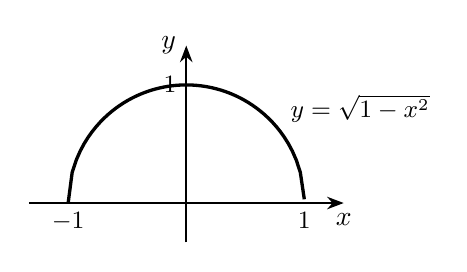
\begin{tikzpicture}
  % Axes
  \draw[axis] (-2,0) -- (2,0) node[below] {$x$};
  \draw[axis] (0,-0.5) -- (0,2) node[left] {$y$};

  % Semicircle
  \draw[very thick, domain=-1:1, samples=60] plot ({1.5*\x}, {1.5*sqrt(1-\x*\x)});

  % Labels
  \node[below, font=\small] at (-1.5,0) {$-1$};
  \node[below, font=\small] at (1.5,0) {$1$};
  \node[left, font=\small] at (0,1.5) {$1$};

  % Label
  \node[right, font=\small] at (1.2,1.2) {$y = \sqrt{1-x^2}$};
\end{tikzpicture}
\end{document}
